\documentclass[11pt,letterpaper]{article}
\usepackage[utf8]{inputenc} %Codificacion del texto (ISO Latin1 encoding)

\usepackage{fancyhdr} %Permite acomodar a tu gusto la parte de arriba y
\usepackage[spanish]{babel} %Permite definir el idioma del dcumento
\usepackage{graphicx} %Permite exportar imagenes en formato eps
\usepackage{url} %Tipo de fuente para correos y paginas
\usepackage{hyperref}
\usepackage{pgf}
\usepackage{fleqn}
\usepackage{amssymb}
\usepackage{fancyvrb}
\usepackage{sectsty}
\usepackage{makeidx}
\usepackage{colortbl} %Permite colocar colores a las tablas
\usepackage{booktabs}
%Margenes%
\parskip 1mm %Espacio entre parrafos

\setlength{\topmargin}{0pt}

\oddsidemargin	0.5cm  % Ancho Letter 21,59cm
\evensidemargin 0.5cm  % Alto  Letter 27,81cm
\textwidth	15.5cm
\textheight	21.0cm
\headsep	4 mm
\parindent	0.5cm
\pagestyle{fancyplain}
\lhead{Informática y Sociedad} %Parte superior izquierda
\rhead{\bf \it Informe de Avances I} %Parte superior derecha
\lfoot{\it Influencia de las tecnologías de la información en colaboraciones
internacionales }
\cfoot{} %Parte inferior central
\rfoot{\bf \thepage} %Parte inferior derecha
\renewcommand{\footrulewidth}{0.4pt} %Linea de separacion inferior

\newtheorem{theorem}{Theorem}
\newtheorem{acknowledgement}[theorem]{Acknowledgement}
\newtheorem{algorithm}[theorem]{Algorithm}
\newtheorem{axiom}[theorem]{Axiom}
\newtheorem{case}[theorem]{Case}
\newtheorem{claim}[theorem]{Claim}
\newtheorem{conclusion}[theorem]{Conclusion}
\newtheorem{condition}[theorem]{Condition}
\newtheorem{conjecture}[theorem]{Conjecture}
\newtheorem{corollary}[theorem]{Corollary}
\newtheorem{criterion}[theorem]{Criterion}
\newtheorem{definition}[theorem]{Definition}
\newtheorem{example}[theorem]{Example}
\newtheorem{exercise}[theorem]{Exercise}
\newtheorem{lemma}[theorem]{Lemma}
\newtheorem{notation}[theorem]{Notation}
\newtheorem{problem}[theorem]{Problem}
\newtheorem{proposition}[theorem]{Proposition}
\newtheorem{remark}[theorem]{Remark}
\newtheorem{solution}[theorem]{Solution}
\newtheorem{summary}[theorem]{Summary}
\newenvironment{proof}[1][Proof]{\noindent\textbf{#1.} }{\ \rule{0.5em}{0.5em}}

\newcommand{\primaria}[1]{
	\textbf{\underline{#1}}
}

\newcommand{\foranea}[1]{
	\textbf{\textsl{#1}}
}

\newcommand{\primyfor}[1]{
	\underline{\foranea{#1}}
}

\makeatletter
\newcommand\subsubsubsection{\@startsection {paragraph}{1}{\z@}%
                                   {-3.5ex \@plus -1ex \@minus -.2ex}%
                                   {1.5ex \@plus.2ex}%
                                   {\normalfont\bfseries}}
\newcommand\subsubsubsubsection{\@startsection {subparagraph}{1}{\z@}%
                                   {-3.5ex \@plus -1ex \@minus -.2ex}%
                                   {1.5ex \@plus.2ex}%
                                   {\normalfont\bfseries}}


\makeatother
%\makeindex
\bibliographystyle{plain}

\begin{document}

%%%%%%%%%%%%%%%%%%%%%%%%%%
%Definicion de la portada%
%%%%%%%%%%%%%%%%%%%%%%%%%%
\begin{titlepage}
    \begin{center}
	%\begin{tabular}{ccc}
	\begin{tabular}{c}
		
\includegraphics[width=0.9\textwidth]{img/logos}
		
	   % 
\includegraphics[width=3cm]{img/utfsm}
	   % & 
	   % \hspace{-0.2cm}
	   % \begin{tabular}{c}
	   % Universidad Técnica Federico Santa María \\ \hline
	   % \vspace{0.2cm}
	   % Departamento de Informática\\
	   % \vspace{1.2cm}
	   % \end{tabular}
	   % \hspace{0.2cm}
	   % &
        %    
\includegraphics[width=2cm]{img/di}
	\end{tabular}

	\vspace{4cm}
	%Titulo del Documento
	\begin{tabular}{c}
		\vspace{3cm}
		\Large{\sc{Seminario de Modelos y Métodos Cuantitativos}}\\
		\huge{\sc{Tarea 2}}\\\\
		%\includegraphics[scale=0.7]{img/portada} \\\\
	\end{tabular}

    \vspace{5cm}
	\begin{tabular}{lr}
			\textbf{Alumnos} & \\
							 & \\
         	\normalsize{Cristián Maureira Fredes} & \url{cmaureir@csrg.inf.utfsm.cl}\\
         	\normalsize{Gabriel Zamora Nelson} & \url{gzamora@csrg.inf.utfsm.cl}\\

							 & \\
			\textbf{Profesor} & \\
							 & \\
         	\normalsize{Andrés Moreira} & \url{amoreira@inf.utfsm.cl}\\
	\end{tabular}

\vspace{2cm}

	%Fecha
    \normalsize{\sc{\today}}\\
    %\normalsize \textbf{Fecha de Entrega:} & {14 de Noviembre del 2010}\\
    \end{center}
\end{titlepage}

\tableofcontents
\newpage

\section{Introducción}
\label{sec:introduccion}
\frame
{
\frametitle{Introducción}
\begin{itemize}
	\item Motivación del problema.
	\item Sobre la técnica.
	\item Implementación inicial.
	\item Sintonización.
	\item \blue{Control}.
	\item Resultados.
\end{itemize}
}



\section{Antecedentes}
\label{sec:antecedentes}
\subsection{Público Objetivo}

\subsubsection{Descripción}
El público objetivo para el presente estudio, se compone principalmente
por personas que se encuentren realizando proyectos de carácter internacional, 
los cuales debido a su distribución geográfica, no les permite una comunicación
relativamente fluida. Además de verse forzosamente necesitados de medios de
comunicación para suplir la distancia. Por otro lado, el no presentar
importancia el área de dichos proyectos e idioma en que se lleve a cabo.

\subsubsection{Información existente}
% Estube buscando alguna publicación/página que hable de la cultura
% americana/alemana, pero no he logrado encontrar nada util =/.

%sobre las herramientas para el trabajo colaboratio
Existen organizaciones que ya han experimentado con herramientas para el
trabajo colaborativo en linea para mejorar la fluidez del intercambio de la
información entre todos sus miembros~\cite{herramientas_trabajo_colaborativo}.
Uno de estas es el uso de wikis. Las wikis~\cite{wikis} son sitios web cuyas
páginas pueden ser editadas por múltiples personas desde un navegador web,
permitiendo redactar documentos colectivamente, siendo ampliamente usadas hoy
en día. El caso más emblemático es el de la wikipedia\cite{wikipedia},
enciclopedia virtual para compartir el conocimiento, editada por voluntarios
de todas las partes del mundo.
Algunos de los softwares más utilizados para ello son
MediaWiki~\cite{mediawiki}, MoinMoin~\cite{moinmoin} y Twiki~\cite{twiki}.
Otros tipos de herramientas utilizadas para la coordinación de diferentes equipos
de trabajo son las herramientas de Software Configuration Management
(SCM~\cite{scm}). Normalmente son utilizadas en actividades de desarrollo de
software, y permiten tratar y controlar la elaboración de código fuente por
varios desarrolladores simultáneamente, pudiendo realizar un seguimiento del
estado de las versiones y sus cambios. Algunas de las herramientas más utilizadas para
esto son Git~\cite{git}, un sistema de control de versiones distribuido,
Subversion (SVN~\cite{svn}), un sistema de control de versiones centralizado,
y  Trac~\cite{trac}, sistema que integra una wiki y sistemas de control de
versiones como Git y SVN, y posee múltiples plugins~\cite{plugin} para
extenderle nuevas funcionalidades.



\subsection{Dominio de la Investigación}

\subsubsection{Descripción}
Con respecto al dominio de la presente investigación, son dos distintas
instancias donde personas de Estados Unidos, Alemania y Chile se reunen
a discutir temáticas en relación al proyecto ALMA:

\begin{itemize}
	\item ACS Weekly Meeting: Reunión donde asisten los colaboradores
(desarrolladores) más importantes del proyecto ALMA, la cual es coordinada
 desde Garching, Alemania.
	\item OSF Coordination Meeting: Reunión en la cual acuden personas de Nuevo
México (EEUU), Garching (Alemania) y Valparaíso (Chile), la cual es 
coordinada por los representantes del grupo ALMA-UTFSM. En ella se plantean temas
de interés general.
\end{itemize}

El dominio de investigación trata sobre que será medido en el corto y largo plazo, 
con respecto a la influencia que tienen las tecnologías de la información en la forma
de trabajo mencionado anteriormente. Se tratará de enfocar los resultados en relación
a objetivos a corto plazo como lo son estados de avances en tareas específicas, para 
medir en que manera influyen las tics en una comunicación de avances de manera fluida e 
intercultural. A largo plazo se medirá a nivel de colaboración el grado de cohesión que 
estas organizaciones logran gracias a la influencia de las tics, refiriéndonos a cantidad
de proyectos logrados con éxito y creación de instancias colaborativas.

\subsubsection{Información existente}

A nuestra investigación le interesan los temas de la comunicación y las
relaciones interpersonales. El dominio es bastante amplio, desde el estudio de
la comunicación oral y corporal la construcción de las relaciones
interpersonales que forman a los grupos de trabajo tanto como las tecnologías
existentes para suplir o complementar a los medios de comunicación.
Dentro de estos ámbitos, existen investigaciones\cite{obs_collaborative} que
han concluido dentro de la información transmitida en las comunicaciones
interpersonales, el lenguaje corporal, el uso de gestos, manos y la forma en
cada persona gesticula transmite significativa información adicional, y cómo
el espacio en el cual se están comunicando influye en las relaciones de
trabajo.

En el trabajo colaborativo desarrollado entre diferentes grupos separados
geográficamente, el tipo de visibilidad que halla de los demás, el moverse
dentro del mismo ambiente compartido, el estar presentes al mismo tiempo, la
audibilidad, tangibilidad y simultaneidad son claramente diferentes al estar
limitados a la comunicación utilizando los medios que las tecnologías nos
ofrecen para ello. Como afecta cada uno de estos factores a la forma de
organización y la forma de trabajo a desarrollar ha sido
estudiada~\cite{proximity_collaboration} concluyendo que, aunque las personas
presentan una mayor facilidad para relacionarse en ambientes de proximidad
física, es posible para las personas colaborar a través de la distancia,
usando cualquier tecnología que tengan disponible. Las personas son capaces de
adaptarse a los medios que disponen, con cierto grado de aceptación, para poder
lograr la comunicar lo que desean. Además, se concluye que el medio de
comunicación utilizado cambia la naturaleza de la comunicación y la naturaleza
de la comunicación, pudiendo pasar de una comunicación menos social a una
enfocada a los tópicos a tratar.

Hoy en día los ambientes de trabajo en el mundo laboral no son lo mismo que
hace años atrás. Tradicionalmente los empresarios han organizado el trabajo de
forma centralizada, sin importar del tipo de trabajo llevado a cabo por cada
uno de los miembros de la empresa. Ahora, la tendencia es la descentralización
e individualización de las diferentes funciones desarrolladas, refiriéndose
con ello a la división de las funciones en los individuos de un grupo de
trabajo, a la delegación y la subdivisión de las diferentes tareas a
realizar por una empresa.
Por ello, mantener una comunicación fluida que evite la pérdida de
identificación de cada trabajador con los objetivos de la empresa o grupo de
trabajo se vuelve de suma importancia.
Para poder evitar estas situaciones, se espera encontrar similitudes que
permitan mejorar las falencias de los modelos de trabajo y la distanciación de
sus identidades con la del grupo de trabajo\cite{trabajo_flexible}.

También se cuenta con la experiencia vivida por el grupo ALMA-UTFSM durante
su formación y desarrollo\cite{utfsm_alma}, en donde se analiza los cambios
que experimentó durante la maduración de su modelo organizacional, donde las
tecnologías de la información determinaron en gran medida las formas de
trabajo colaborativas llevadas a cabo. Se destacan las variables del ambiente
que lograron alcanzar el éxito del grupo, las cuales se deben analizar en
conjunto para entender la real importancia de cada una de ellas. El tener estudiantes
entusiastas y motivados, seleccionados tanto por sus habilidades sociales como
técnicas, y un grupo docente involucrado, que les guía y da soporte, permite
que se fomente la proactividad y que los proyectos estén en
continuo desarrollo.



\section{Análisis y Resultados de Antecedentes}
\label{sec:analisis}
Se describen a continuación los análisis a distintos factores que hemos
decidido como equipo, que son dignos de estudiar.

\subsection{Idioma}
Es conocido que el idioma universal, nos guste o no,
es el inglés, por lo tanto al momento de participar en
cualquier reunión con personas de distintos países,
la única solución es poder comunicarnos con dicho lenguaje.

Por lo tanto cada miembro presente, debe preocuparse no tanto
por saber la traducción de palabras en español al inglés,
sino en algo mucho más complejo, saber expresar las ideas
en un lenguaje distinto que el idioma del país natal.

%Agregar más

\subsection{Zonas Horarias}
Si bien es cierto, para cualquier persona, fijar una reunión
a una cierta hora no es una tarea difícil, tenemos que darnos
cuenta que al momento de pensar en una reunión internacional,
la mayoría de los países poseen una zona horaria distinta, por
lo cual, las personas encargadas tanto de organizar como de
participar en alguna reunión de esa índole, debe poseer el
conocimiento del horario de los países en cuestión,
y saber cuantas horas de diferencia se tienen, pues, mientras
en un lugar el día puede estar comenzando, el otro, puede estar
acabando.

Actualmente en dichas reuniones, uno de los mayores problemas
que se han tenido, son las diferencias muy grandes entre EEUU, 
Alemania y Chile, pues si tomamos en consideración a Chile,
EEUU tiene 2 horas menos y Alemania tiene 6 horas más, lo cual
claramente es un problema, pues se necesita encontrar un balance.
%Agregar más

\subsection{Costumbres}
Es conocido de que lamentablemente en Chile, nos caracterizamos
por ser un poco impuntuales, independiente de si se trata de una
reunión formal, a una fiesta de cumpleaños. Por lo que debido a lo
anteriormente señalado, en todos los países hay distintas costumbres
y es en la puntualidad que nos hemos fijado, en el cual Alemania
destaca por cumplir su palabra completamente, pues al momento
de iniciar una reunión, si es a las 11:00 am, no es ni un par
de minutos antes ni un par de minutos después, pero lamentablemente
tanto en EEUU como en Chile, ocurre lo contrario.

Es por lo anteriormente señalado que cada vez que se comienza una
reunión ocurren los problemas de ``Estamos esperando a una persona
para poder comenzar.''

\subsection{Experiencia Técnica}
Si bien es cierto, expresar las ideas en otro idioma, no es algo
trivial que se le dé innatamente a cualquier persona, para participar
en distintas reuniones donde se discuten temáticas de una índole técnica
es necesario tener el conocimiento técnico necesario para, aparte de
entender la idea que la otra persona está queriendo expresar, entender
que significa lo que está diciendo.
Es por ésto, que las personas que participan en las reuniones,
es gente que conoce lo que es ACS (ALMA Common Software) a un nivel
intermedio, para poder sobrevivir en un lugar donde se discutan ideas
en torno al dicho software.
%Agregar más

\subsection{Medios de comunicación}
Cuando uno realiza teleconferencias con distintas personas,
nunca al finalizar, quedan todas las ideas completamente claras,
o mirado desde otro punto de vista, siempre hay nuevos temas
o dudas respecto a lo que se habló, por lo cual es necesario
comunicarse con las personas que plantearon dicha idea, o que
simplemente están a cargo.

Para poder realizar una comunicación más fluida entonces,
es necesario tener otros medios para poder comunicarnos,
es decir, aparte de Skype~\cite{Skype} para realizar
dichas teleconferencias, se necesitan otras formas, como lo son:
\begin{itemize}
   \item Mensajería Instantánea: Es necesario establecer un protocolo de comunicación
		único para dicho objetivo, en el cual se pueda agregar a las personas de interés, logrando
		una interacción rápida y expedita. En nuestro caso se utiliza Yahoo Messenger.
   \item Correo Electrónico: Si bien es cierto existen las reuniones, es necesario también
		poder tener una comunicación un poco indirecta para comentar problemas, o presentar
		avances de un cierto trabajo a todas las personas interesadas mediante listas de correo.
   \item Acceso Telefónico: Las reuniones se realizan mediante teleconferencias, por lo cual
		es necesario tener acceso telefónico con el extranjero, o en el caso nuestro, poder
		contar con una cuenta Skype para llamadas a todo el mundo.
\end{itemize}

\subsection{Medios de almacenamiento de información}
Para cada reunión apropiadamente desarrollada,
es necesario poseer una minuta para tener un orden
cronológico de los temas a tratar o el orden
en que las personas tienen la palabra, para poder
expresar sus ideas y consultas.

Por lo tanto es muy positivo, que todas las personas
estén familiarizadas con dichos medios, en este caso hablamos
de TWiki (referencia a la TWiki), un medio de almacenamiento
comunitario de comunicación, que es utilizado tanto como para
presentar las minutas, como para el desarrollo de los distintos
proyectos colaborativos alrededor de lo que es ACS.

%Agregar mas

\subsection{Relación con Tecnologías de la Información}

Si nos damos cuenta, en todos los puntos señalados anteriormente
la tecnología juega un papel fundamental, ya sea desde el
almacenamiento de información, como para una comunicación directa.

% Agregar mas


\newpage
\bibliography{paper,url}

\section{Anexos}
\label{sec:anexos}
% Agregar:
% antecedentes recolectados
% otros (imágenes, textos, tablas, etc.)




\subsection{Actividades y tiempos empleados por cada integrante}

\begin{tabular}{|l|p{7cm}|c|}
\hline
Integrante & Actividades & Tiempo Empleado \\\hline
Cristián Maureira & Observación de los medios de comunicación y reuniones internacionales. & 7 horas \\
& Creación del Repositorio de trabajo. & 30 minutos \\
& Creación del esqueleto del informe.& 30 minutos \\
& Desarrollo de la introducción. & 2.5 horas \\
& Redacción de los análisis y resultados de antecedentes. & 3 horas \\
& Revisión de los análisis y resultados de antecedentes. & 1 hora \\
\hline
Gabriel Zamora & Revisión de  las formas de trabajo de cada grupo. & 8 horas \\
& Estudio del público objetivo y del dominio del trabajo. & 3 horas \\
& Redacción de los análisis y resultados de antecedentes. & 4 horas \\
\hline
Rodrigo Fernández & Comparación de los resultados con los antecedentes
recopilados. & 5 horas \\
& Investigación de la información existente. & 5 horas \\
& Redacción de los análisis y resultados de antecedentes. & 3 horas \\
& Revisión del análisis y resultados de antecedentes. & 30 minutos \\
& Revisión ortográfica del informe. & 10 minutos \\
\hline
\end{tabular}
\newpage
\subsection{Participantes de las reuniones}
\subsubsection{OSF Coordination Meeting}

\begin{tabular}{|l|l|l|l|}
	\hline
	{\bf Nombre} & {\bf Cargo} & {\bf Organización} & {\bf País} \\\hline
	Heiko Sommers & ACS Technical Leader & ESO & Alemania \\\hline
	Gianluca Chiozzi & ESO Astronomical Instrumentation Leader & ESO & Italia \\\hline
	Alessandro Caproni & Software Engineer& ESO & Italia \\\hline
	Matias Mora & Software Engineer & ALMA & Chile \\\hline
	Nicolas Troncoso & Software Engineer & ALMA & Chile \\\hline
	Jorge Avarias & Software Engineer & NRAO & EEUU \\\hline
	Rodrigo Tobar & Software Engineer & ESO & Alemania \\\hline
	Jaime Pavlich & Profesor & UCN & Chile \\\hline
	Tomas Staig & Computer Science Student & UTFSM/ESO & Chile \\\hline
	Arturo Hoffstadt & Computer Science Engineer & UTFSM/NRAO & Chile \\\hline
	Gabriel Zamora & Computer SCience Student & UTFSM & Chile \\\hline
	Cristián Maureira & Computer SCience Student & UTFSM & Chile \\\hline	
\end{tabular}

\subsubsection{ACS Weekly Meeting}

\begin{tabular}{|l|l|l|l|}
	\hline
	{\bf Nombre} & {\bf Cargo} & {\bf Organización} & {\bf País} \\\hline
	Joseph Schwarz & ACS Project Leader & ESO & Alemania \\\hline
	Heiko Sommers & ACS Technical Leader & ESO & Alemania \\\hline
	Gianluca Chiozzi & ESO Astronomical Instrumentation Leader & ESO & Italia \\\hline
	Alessandro Caproni & Software Engineer& ESO & Italia \\\hline
	Jorge Avarias & Software Engineer & NRAO & EEUU \\\hline
	Rodrigo Tobar & Software Engineer & ESO & Alemania \\\hline
	Arne Grimstrup & Software Engineer & NRAO & Canada \\\hline
	Bogdam Jeram & Software Engineer & ESO & Eslovenia \\\hline
	Helmut Tischer & Software Engineer & ESO & Alemania \\\hline
	Matej Sekoranja & Software Engineer  & ESO & Eslovenia \\\hline
	Roberto Cirami & Software Engineer & INAF - OAT & Italia\\\hline
	Tomas Staig & Computer Science Student & UTFSM/ESO & Chile \\\hline
	Gabriel Zamora & Computer Science Student & UTFSM & Chile \\\hline
	Cristián Maureira & Computer Science Student & UTFSM & Chile \\\hline	
\end{tabular}

% CORRECCION 6
\subsubsection{Fotografías}
A continuación se muestran algunas fotografías tomadas mientras se realizaban las reuniones semanales.\\

\begin{center} 
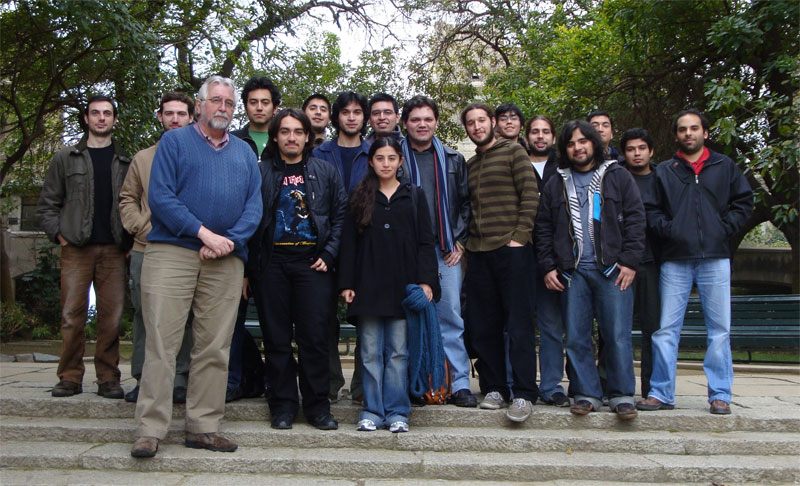
\includegraphics[width=0.8\textwidth]{images/alma-utfsm-1}\\\vspace{1cm}
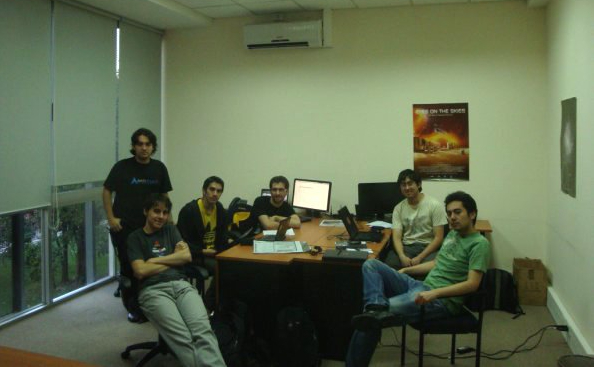
\includegraphics[width=0.8\textwidth]{images/alma-utfsm-2}\\
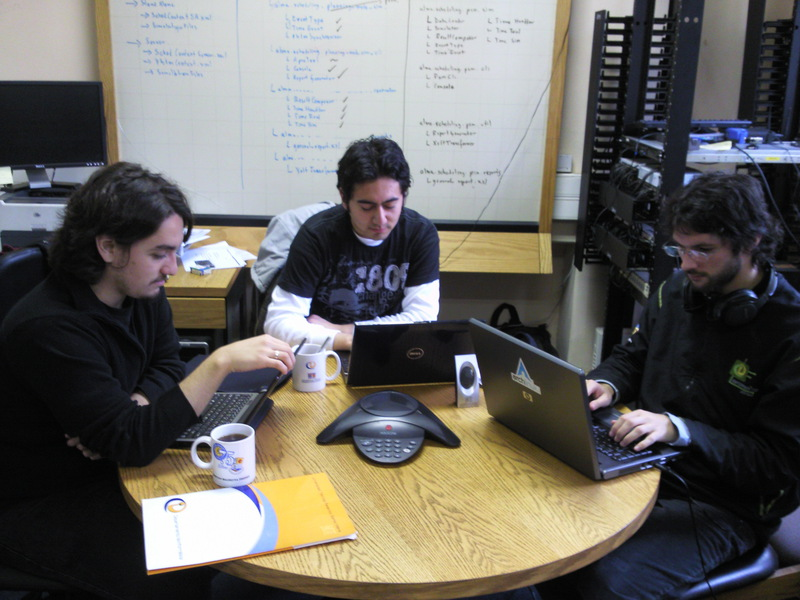
\includegraphics[width=0.8\textwidth]{images/lab_conference}\\\vspace{1cm}
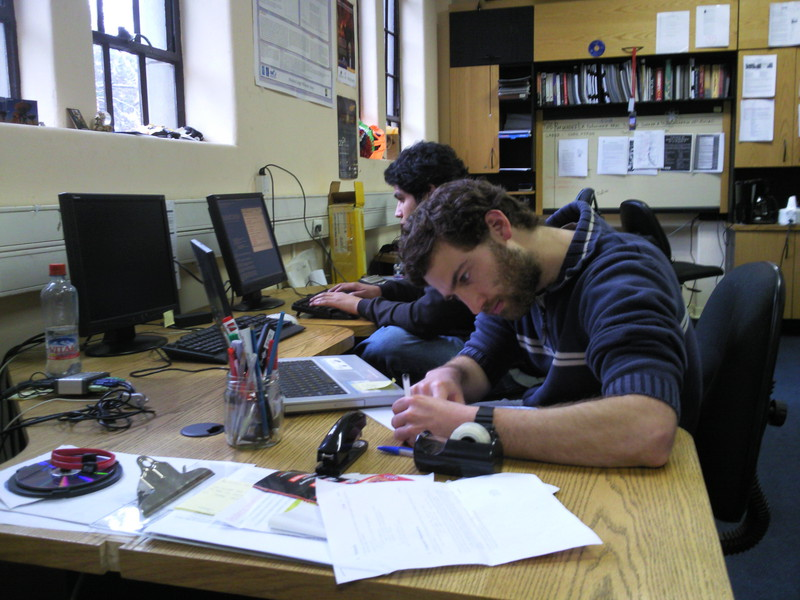
\includegraphics[width=0.8\textwidth]{images/lab_working}\\
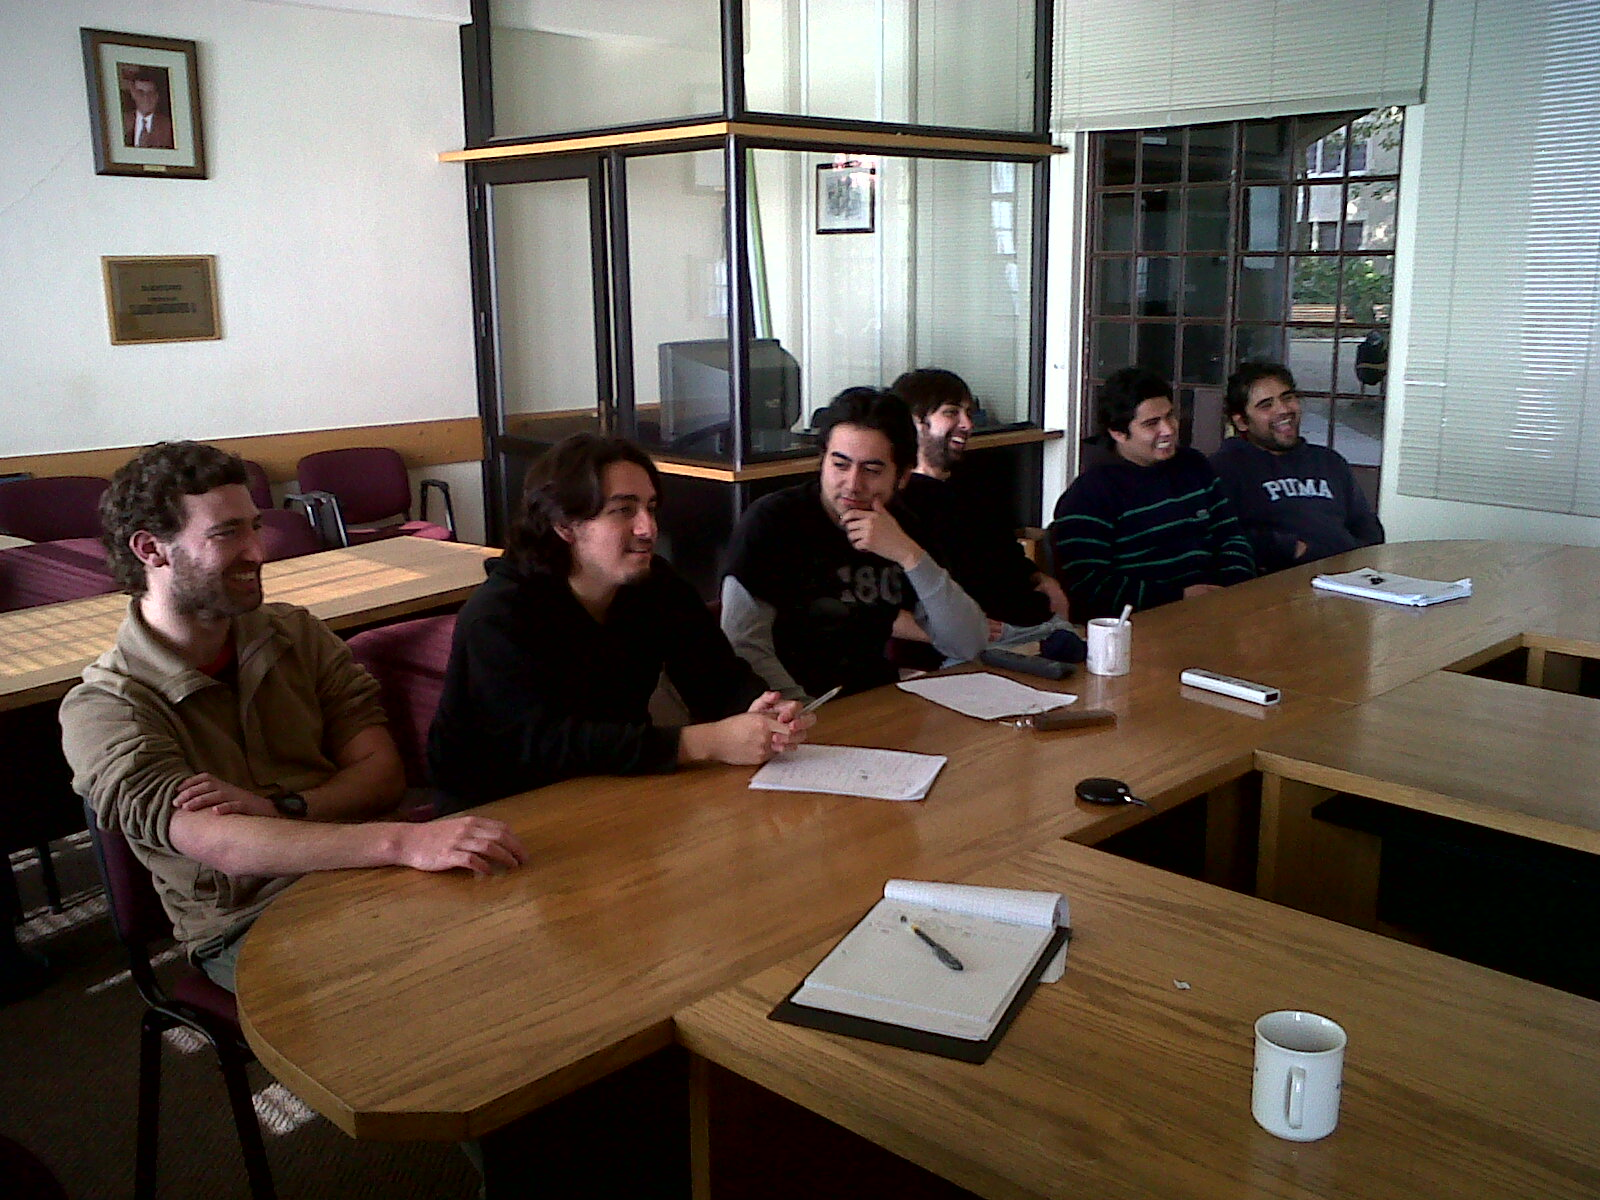
\includegraphics[width=0.8\textwidth]{images/leads1}\\\vspace{1cm}
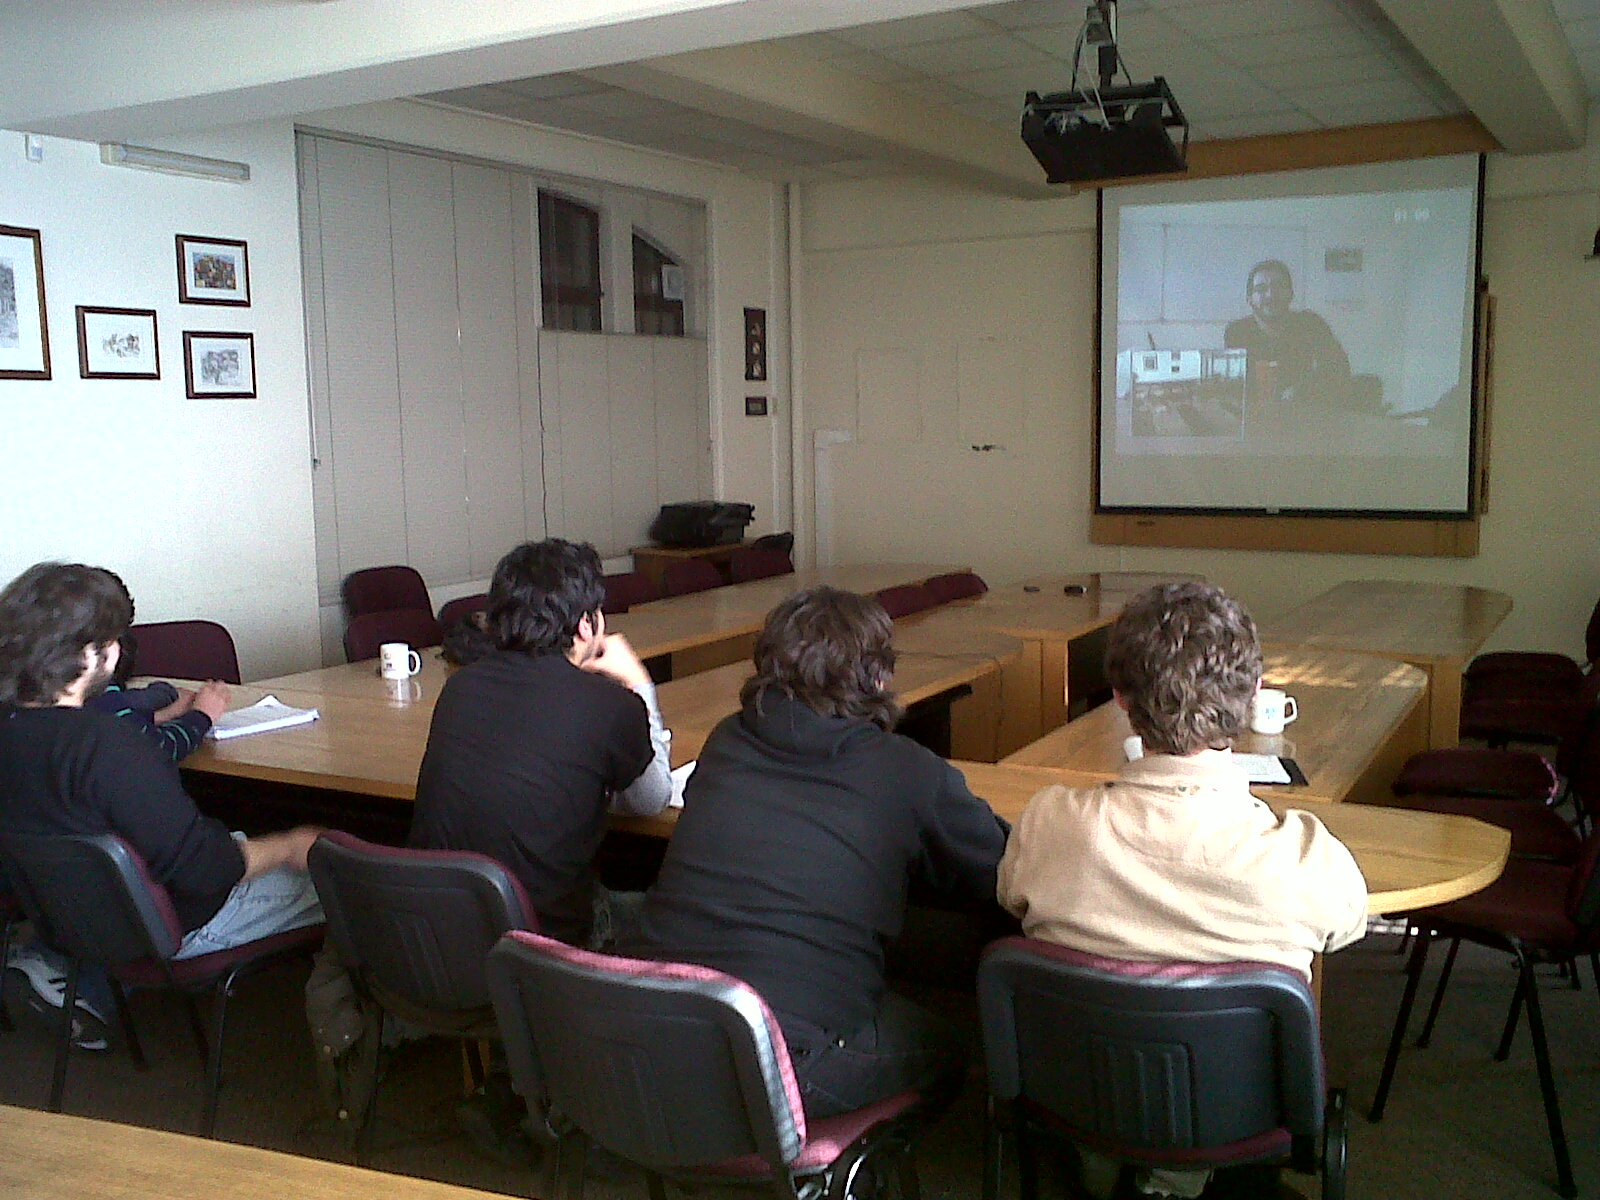
\includegraphics[width=0.8\textwidth]{images/leads2}
\end{center}
% CORRECCION &

\newpage
\subsection{Minutas de reuniones}
\subsubsubsection{ACS Weekly Meeting}
\begin{verbatim}
ACS Weekly Phone Meeting 
Date: Monday, 2010-04-12 

Attendees: 
ESO: Bogdan, Gianluca, Heiko, JosephSchwarz, 
NRAO: ArneGrimstrup, JorgeAvarias 
JSI: 
AOT: 
ALMA Chile: Ale 
UTFSM: GabrielZamora CristianMaureira 

Control contact number: +1-203-607-6471 (Passcode 203403#) 

General issues 

Alma has a promising candidate for a new board to replace the VMEs with 64 
bit architecture, to support more memory. Details from Thomas J. 
All module owners please fix their tests on 8.2 branch and HEAD. 

Ale Caproni 

Last week: 

CONTROL: Some issues with TotalPower testing, also due to STEs gotten messed up 
by other testers. 
The TP component has been changed to use the C++ API of the Bulk data libs, 
without reusing the IDL wrapper of the bulk data component. This works fine 
now, but still would like to discuss changes to the BD IDL for the long term. 
Will be at ESO early May. Things to be discussed should be added to Ale's 
Main.May2010 page.

Arne Grimstrup 

Last week: 

Continued investigation of COMP-3072 (with J. Avarias) 
problem still occurs with RHEL 5.4 version of CASA 
select is monitoring a bad file descriptor which triggers an exception 
in the TAO code. Telecon with UTFSM regarding future projects 
(with G. Chiozzi, H. Sommer, et. al.) Support 
Investigation of 64-bit test faults in NRI (H. Sommer)(with J. Avarias) 
Template method was invoking unsigned long version of getValue method 
that didn't exist Documentation for generated Python bindings (J. Kern) 
Questions regarding Python Binding Generator (J. Kern) 
Problem building ACS in INTROOT (J. Avarias) 

This week: 
Continue work on COMP-3072 
Continue work on COMP-830 

Bogdan Jeram 

Last week: 
Monday public holiday 
4 days of vacation 

Heiko Sommer 

Last week: 

Worked out HibernateDAL's usage of Archive's new archiveConfig.properties 
mechanism, together with Holger. 
Finalized 8.1 CVS logs and release notes. Pre-release of 9.0 VM. 
Discussions, e.g. TP with Ale and others 
Support, e.g. XSD validation, CDB performance fix, manager error messages, 
1 day leave 
Telecon with UTFSM about current projects 
quarterly report for ESO 

Helmut Tischer 

Last week: 
Vacation 

This week: 
COMP-2214 continuing 

Joe Schwarz 

Last week: 

Discussed problem of simultaneous use of SB by > 1 STE; change in 
lifecycle-handling needed 
Reviewed FP6 quarterly report from U. of Cambridge 
Worked on Total Power crash of Java container; suggested JNI 
debugging options for JVM runtime to Jeff and Ville, also removing
 native method invocation from class constructor (this didn't 
make any difference, however); got help from Roberto, who looked 
at logs and said he saw no bulk data issues 
Discussed CDR8 preparations w/Heiko 
Tried (and failed) to convince Brian to take Observation Control 
(not yet delivered) out of R7.1 
One day's leave 

This week: 
CDR8 preparation, ACS 9.0 planning 
Continue investigation of Total Power problem 
Return to classpath generation 

Jorge Avarias 

Last week: 

COMP-3749: ACS to introduce a new log level between DEBUG and TRACE 
Finished to make the last changes to the tests (Changed ACS_LOG_STDOUT 
from 2 to 1 new trace) 
All the tests affected by this are passing. 
Continued investigation of COMP-3072 (with A, Grimstrup) 
Fixed NRI ACS 64 bits building problems: 
The method unsigned long cdb::DAONode::getValue(char const*) 
was missing. probably some code is using unsigned long instead 
CORBA::ULong (in 32 bits they have the same length, in 64 they have not) 
Support: 
CONTROL/ACC/cppContainer crash (T. Powers) 
CONTROL/ACC/javaContainer crash, JVM is crashing with Seg. Fault 
(J. Kern, V. Suoranta) 
Problems building ACS in INTROOT (ACS is already built in ACSROOT) 
(S. Rankin) 


Matej Sekoranja 

Last week: 
HibernateDAL now skips loading all .dtd files, XMLSchema.xsd and xml.xsd so 
that Oracle's XMLTYPE checks don't get confused. 

This week: 
At CERN, but available for emergency ACS work. 

This week: 
TMCDB integration at the OSF 

UTFSM 

Last week: 

DDS Logging Service 
All the main goals are completed 
There are one pending task, write a "state of art" in this topic, for the paper 
accepted in the SPIE Meeting with people at ESO to define project objectives. 
Planning
Python support for BACI Properties 
ACS Code Generation 
ACS Windows Porting (Rodrigo and Heiko to integrate Java porting, Camillo and 
Gianluca to continue with C++ porting)
\end{verbatim}
\newpage
\subsubsubsection{OSF Coordination Meeting}

\begin{verbatim}
Date: Tue, 2010-05-18, 11:00 Chile, 9:00 Socorro, 17:00 Germany 
Attendees: 

ALMA-Chile: MatiasMora 
NRAO-Socorro: JorgeAvarias 
ESO-Garching: HeikoSommers 
UTFSM: GabrielZamora, TomasStaig, ArturoHoffstadt, CristianMaureira 
UCN: JaimePavlich 

Contact Info 
When: 11:00 Chile / 9:00 NM / 17:00 Germany 
Chile (toll free): 800532833 
International: +1 3032480281 
Access Code: 4676238 
Web Conferencing URL: http://net.globalcrossing.com/conferencing/ 

Agenda 
ALMA-CONICYT #31090034 (UTFSM) 
Projects 
ACS Windows Porting: The first version of the gcc-wrapper (gcc -> cl) is 
ready, we need to test with real examples to improve it. 
Code Generation: Luigi sent us a project proposal. Because Luigi was on
 vacations the last week, the meeting for this project is pending 
Alarms Configuration GUI: 
The project is ready, but there are some details with the redaction. 
Rules view that Tomas will fix in the week. 
Cristian Maureira and Tomas Staig will work on the documentation the 
next week. 
Official acceptance by ACS. 
Sampling System GUI: 
Juan Reyes and Cristian Maureira closed two of the three pending bugs, 
there are only one pending, that will be ready during the week. 
Official acceptance by ACS. 
ALMA-CONICYT #31080031 (AIA) 
Teams working on papers and on a new task about implementing TSP with 
their paper techniques 
HPC must to define the input framework and do some testing with TSP 
SebastianDuran and WalterFarina will be helping MatiasMora on what 
he needs for his thesis 
Second class this week Valpo. and next week Stgo. about advanced 
AI techniques 
Looking for possibilities of collaborations with MAIA-INRIA 
Summer Jobs 2010 
Pending reports! 
UCN Current Status 
Mini-ACS-Workshop from April 27th to May 10th. Funded by 
ALMA #31090026. 
Repository for UCN projects: http://goos-acs.googlecode.com 
gCCD status 
Implementing support for SBIG cameras 
Moving configuration to CDB 
gDome status 
gDome group are new students. After several intensive sessions 
they created the first version of the Dome component. 
Documentation: installation and system manuals. 
Misc 
ACS Scientific Linux distribution mirror repo here at UTFSM (ArturoHoffstadt).
\end{verbatim}

\end{document}
